\documentclass[bigtut]{tutorial}\usepackage[]{graphicx}\usepackage[]{color}
%% maxwidth is the original width if it is less than linewidth
%% otherwise use linewidth (to make sure the graphics do not exceed the margin)
\makeatletter
\def\maxwidth{ %
  \ifdim\Gin@nat@width>\linewidth
    \linewidth
  \else
    \Gin@nat@width
  \fi
}
\makeatother

\definecolor{fgcolor}{rgb}{0.345, 0.345, 0.345}
\newcommand{\hlnum}[1]{\textcolor[rgb]{0.686,0.059,0.569}{#1}}%
\newcommand{\hlstr}[1]{\textcolor[rgb]{0.192,0.494,0.8}{#1}}%
\newcommand{\hlcom}[1]{\textcolor[rgb]{0.678,0.584,0.686}{\textit{#1}}}%
\newcommand{\hlopt}[1]{\textcolor[rgb]{0,0,0}{#1}}%
\newcommand{\hlstd}[1]{\textcolor[rgb]{0.345,0.345,0.345}{#1}}%
\newcommand{\hlkwa}[1]{\textcolor[rgb]{0.161,0.373,0.58}{\textbf{#1}}}%
\newcommand{\hlkwb}[1]{\textcolor[rgb]{0.69,0.353,0.396}{#1}}%
\newcommand{\hlkwc}[1]{\textcolor[rgb]{0.333,0.667,0.333}{#1}}%
\newcommand{\hlkwd}[1]{\textcolor[rgb]{0.737,0.353,0.396}{\textbf{#1}}}%
\let\hlipl\hlkwb

\usepackage{framed}
\makeatletter
\newenvironment{kframe}{%
 \def\at@end@of@kframe{}%
 \ifinner\ifhmode%
  \def\at@end@of@kframe{\end{minipage}}%
  \begin{minipage}{\columnwidth}%
 \fi\fi%
 \def\FrameCommand##1{\hskip\@totalleftmargin \hskip-\fboxsep
 \colorbox{shadecolor}{##1}\hskip-\fboxsep
     % There is no \\@totalrightmargin, so:
     \hskip-\linewidth \hskip-\@totalleftmargin \hskip\columnwidth}%
 \MakeFramed {\advance\hsize-\width
   \@totalleftmargin\z@ \linewidth\hsize
   \@setminipage}}%
 {\par\unskip\endMakeFramed%
 \at@end@of@kframe}
\makeatother

\definecolor{shadecolor}{rgb}{.97, .97, .97}
\definecolor{messagecolor}{rgb}{0, 0, 0}
\definecolor{warningcolor}{rgb}{1, 0, 1}
\definecolor{errorcolor}{rgb}{1, 0, 0}
\newenvironment{knitrout}{}{} % an empty environment to be redefined in TeX

\usepackage{alltt}
\unitcode{MATH1005}
        \unitname{Statistics}
        \semester{Summer/Winter/Semester2}
        \sheetnumber11

\usepackage{graphicx}
%\withsolutions
\IfFileExists{upquote.sty}{\usepackage{upquote}}{}
\begin{document}
\lettersfirst

\begin{tutorial}

\begin{center}
\begin{tabular}{| ll |} \hline
& \\
{\bf 1 Sample Z Test} & \\
Context & $n$ observations from  a population with unknown mean $\mu$ and known variance $\sigma^2$ \\
Hypothesis &   $H_{0}: \mu = \mu_{0}$   \\
Test Statistic & $\tau =   \frac{  \bar{X} - \mu_{0}  } {  \frac{  \sigma }{ \sqrt{n}  }}      \overset{H_0}{\sim} N(0, 1)$      \\ 
& \\  \hline
\end{tabular}
\end{center}


\begin{center}
\begin{tabular}{| ll |} \hline
& \\
{\bf 1 Sample t Test} & \\
Context & $n$ observations from  a population with unknown mean $\mu$ \\
& and unknown variance $\sigma^2$ \\
Hypothesis &   $H_{0}: \mu = \mu_{0}$   \\
Test Statistic & $\tau =   \frac{  \bar{X} - \mu_{0}  } {  \frac{  s }{ \sqrt{n}  }}      \overset{H_0}{\sim} t_{n-1}$      \\ 
& \\  \hline
\end{tabular}
\end{center}

\begin{center}
\begin{tabular}{| ll |} \hline
& \\
{\bf 2 Sample t Test} & \\
Context & 2 populations with unknown means $\mu_{X}$ and  $\mu_{Y}$  \\
&  and unknown variances $\sigma_{X}^2$ and $\sigma_{Y}^2$ \\
& 2 samples $\{ X_i \} $ and $\{ Y_j \} $ of size $n_x$ and $n_y$ \\
Hypothesis &   $H_{0}: \mu_X - \mu_Y = 0$   \\
Test Statistic & $\tau =   \frac{  \bar{X} - \bar{Y} - 0  } {  s_p  \sqrt{ \frac{1}{n_x} +  \frac{1}{n_y}  }}      \overset{H_0}{\sim} t_{n_x + n_y-2}$      \\ 
&  \hspace{2cm}    where \;   $s_p^2 =  \frac{   (n_x-1) s_x^2 + (n_y-1) s_y^2 }{ n_x + n_y -2 }$ \;\; \\
& \\  \hline
\end{tabular}
\end{center}

\vspace{.5cm}
\begin{questions}

\question  Breaking strenth of rope \\

The breaking strengths of ropes produced by a
manufacturer have mean 1800N and standard deviation 100N. By a
new technique in the manufacturing process, it is claimed that the
breaking strength can be increased without changing the variability.
To test this claim a sample of 50 ropes is tested and it is found that the mean breaking strength
is 1850N. Can you support the manufacturer's claim? Justify your
decision using a statistical argument. \\

Let $X_{i} \;\; i=1,\ldots,50$ be the breaking strengths and let $\mu$ be the population mean of the ropes produced by the new technique. \\

\begin{parts}
\part Hypothesis: Explain why a one-sided test of $H_0: \mu=1800  \;\; vs \;\; H_1: \mu>1800$ is suitable to test the manufacturer's claim. \\

\part Assumptions: Are the assumptions for a Z test valid  here? \\

 \part Test statistic: What is the test statistic and its distribution under $H_{0}$? \\
 
\part P-value: Calculate the p-value using the Normal tables and R. 

\begin{knitrout}
\definecolor{shadecolor}{rgb}{0.969, 0.969, 0.969}\color{fgcolor}\begin{kframe}
\begin{alltt}
\hlnum{1}\hlopt{-}\hlkwd{pnorm}\hlstd{(}\hlnum{1850}\hlstd{,}\hlnum{1800}\hlstd{,}\hlnum{100}\hlopt{/}\hlkwd{sqrt}\hlstd{(}\hlnum{50}\hlstd{))}
\end{alltt}
\end{kframe}
\end{knitrout}

 \part Conclusion: Draw your conclusion based on the p-value. \\
 
 \part It is found that the sample of breaking strengths has standard deviation 110N. Now use a $t$ Test, and compare your results.
 
\begin{knitrout}
\definecolor{shadecolor}{rgb}{0.969, 0.969, 0.969}\color{fgcolor}\begin{kframe}
\begin{alltt}
\hlstd{t}\hlkwb{=}\hlstd{(}\hlnum{1850}\hlopt{-}\hlnum{1800}\hlstd{)}\hlopt{/}\hlstd{(}\hlnum{110}\hlopt{/}\hlkwd{sqrt}\hlstd{(}\hlnum{50}\hlstd{))}
\hlnum{1}\hlopt{-}\hlkwd{pt}\hlstd{(t,}\hlnum{49}\hlstd{)}
\end{alltt}
\end{kframe}
\end{knitrout}
\end{parts}


\begin{solution}
Let $X_{i} \;\; i=1,\ldots,50$ be the breaking strengths and let $\mu$ be the population mean of the ropes produced by the new technique.
We have a sample with $n=50$ and $\bar{x}=1850$. \\

\fbox{H}
$H_0: \mu=1800  \;\; vs \;\; H_1: \mu>1800$ \\
This one-sided test is suitable as  the manufacturer claims that rope strength has {\it increased}. \\

\fbox{A} 
$\sigma^2 = 100^2$ is known (`new technique ... without changing the variability'). \\

 \fbox{T}
$\tau = \bar{X} \overset{H_0}{\sim} N(1800,100^2/50)$. \\
Observed value: $\bar{x} = 1850$. \\

OR in standardised form: \\

$\tau = \frac{ \bar{X} - 1800}{\frac{100}{\sqrt{50}} } \overset{H_0}{\sim} N(0,1) = Z$. \\
Observed value: $\tau_{0} = \frac{1850-1800}{\frac{100}{\sqrt{50}} } = 3.535534 $ \\


\fbox{P} \\

Using Normal Tables: \\
$\text{P-value} = P( Z > 3.535534) = 1-P(Z < 3.54) = 0.0002$. \\

Using R:
\begin{knitrout}
\definecolor{shadecolor}{rgb}{0.969, 0.969, 0.969}\color{fgcolor}\begin{kframe}
\begin{alltt}
\hlnum{1}\hlopt{-}\hlkwd{pnorm}\hlstd{(}\hlnum{1850}\hlstd{,}\hlnum{1800}\hlstd{,}\hlnum{100}\hlopt{/}\hlkwd{sqrt}\hlstd{(}\hlnum{50}\hlstd{))}
\end{alltt}
\begin{verbatim}
## [1] 0.000203476
\end{verbatim}
\begin{alltt}
\hlnum{1}\hlopt{-}\hlkwd{pnorm}\hlstd{(}\hlnum{3.54}\hlstd{)}
\end{alltt}
\begin{verbatim}
## [1] 0.0002000635
\end{verbatim}
\end{kframe}
\end{knitrout}

\vspace{.5cm}
\fbox{C}
Since $\text{p-value}$ is small, we strongly reject $H_{0}$. \\
There appears to be strong evidence that the rope strength has increased.

\vspace{1cm}
Now repeating using a t test, where $n=50$ and $s=110$.\\

\fbox{H}
$H_0: \mu=1800  \;\; vs \;\; H_1: \mu>1800$ \\

\fbox{A} 
We assume that the population is Normally distributed. \\

 \fbox{T}
$\tau = \frac{ \bar{X} - 1800}{\frac{s}{\sqrt{50}} } \overset{H_0}{\sim} t_{49}$. \\
Observed value: $\tau_{0} = \frac{1850-1800}{\frac{110}{\sqrt{50}} } = 3.214122 $ \\


\fbox{P} \\

Using $t_{50}$ Table (as closest): \\
$\text{P-value} = P( t_{49} > 3.214122) \approx P( t_{50} > 3.214122) \in (0.001,0.0025)$. \\

Using R:
\begin{knitrout}
\definecolor{shadecolor}{rgb}{0.969, 0.969, 0.969}\color{fgcolor}\begin{kframe}
\begin{alltt}
\hlnum{1}\hlopt{-}\hlkwd{pt}\hlstd{(}\hlnum{3.214122}\hlstd{,}\hlnum{49}\hlstd{)}
\end{alltt}
\begin{verbatim}
## [1] 0.001158165
\end{verbatim}
\end{kframe}
\end{knitrout}

\vspace{.5cm}
\fbox{C}
Since $\text{p-value}$ is small, we strongly reject $H_{0}$. \\
There appears to be strong evidence that the rope strength has increased.
\end{solution}



\question Paired t Test \\

In order to test the difference between two drugs A and B for treatment of high blood pressure, 24 patients are paired according to age. One of each pair is chosen at random to receive drug A and the other receives drug B. 
The resultant drops in blood pressure are set out below:

\begin{center}
\begin{tabular}{| l | l | l | l | l | l | l | l | l | l | l | l | l |} \hline
Pair & 1 & 2 & 3 & 4 & 5 & 6 & 7 & 8 & 9 & 10 & 11 & 12 \\ \hline
Drug A & 5 & 4 & 2 & 6 & 9 & 1  &1 & 5  & 6 & 3 & 7 & 14 \\ 
Drug B & 2 & 5 & 1  & 2  &6 & 3 & 0  & 2 & 5 & 2  & 7 & 12 \\ \hline
Difference & & & & & & & & & & & & \\ \hline
\end{tabular}
\end{center}

\vspace{.5cm}
\begin{parts}
\part Fill in the row:  Difference = Drug A - Drug B.   

\begin{knitrout}
\definecolor{shadecolor}{rgb}{0.969, 0.969, 0.969}\color{fgcolor}\begin{kframe}
\begin{alltt}
\hlstd{a} \hlkwb{=}\hlkwd{c}\hlstd{(}\hlnum{5}\hlstd{,}\hlnum{4}\hlstd{,}\hlnum{2}\hlstd{,}\hlnum{6}\hlstd{,}\hlnum{9}\hlstd{,}\hlnum{1}\hlstd{,}\hlnum{1}\hlstd{,}\hlnum{5}\hlstd{,}\hlnum{6}\hlstd{,}\hlnum{3}\hlstd{,}\hlnum{7}\hlstd{,}\hlnum{14}\hlstd{)}
\hlstd{b}\hlkwb{=}\hlkwd{c}\hlstd{(}\hlnum{2}\hlstd{,}\hlnum{5}\hlstd{,}\hlnum{1}\hlstd{,}\hlnum{2}\hlstd{,}\hlnum{6}\hlstd{,}\hlnum{3}\hlstd{,}\hlnum{0}\hlstd{,}\hlnum{2}\hlstd{,}\hlnum{5}\hlstd{,}\hlnum{2}\hlstd{,}\hlnum{7}\hlstd{,}\hlnum{12}\hlstd{)}
\hlstd{diff}\hlkwb{=}\hlstd{a}\hlopt{-}\hlstd{b}
\end{alltt}
\end{kframe}
\end{knitrout}

\part Calculate the mean and standard deviation of the differences. 

\begin{knitrout}
\definecolor{shadecolor}{rgb}{0.969, 0.969, 0.969}\color{fgcolor}\begin{kframe}
\begin{alltt}
\hlkwd{mean}\hlstd{(diff)}
\hlkwd{sd}\hlstd{(diff)}
\end{alltt}
\end{kframe}
\end{knitrout}

\part Perform a t test for $H_0: \mu_d = 0$, where $\mu_d$ is the population mean of differences. 

\begin{knitrout}
\definecolor{shadecolor}{rgb}{0.969, 0.969, 0.969}\color{fgcolor}\begin{kframe}
\begin{alltt}
\hlstd{t}\hlkwb{=}\hlkwd{mean}\hlstd{(diff)}\hlopt{/}\hlstd{(} \hlkwd{sd}\hlstd{(diff)}\hlopt{/}\hlkwd{sqrt}\hlstd{(}\hlkwd{length}\hlstd{(diff)) )}
\hlnum{2}\hlopt{*}\hlstd{(}\hlnum{1}\hlopt{-}\hlkwd{pt}\hlstd{(t,}\hlkwd{length}\hlstd{(diff)}\hlopt{-}\hlnum{1}\hlstd{))}
\end{alltt}
\end{kframe}
\end{knitrout}

\part Produce a boxplot of the differences.  Comment. 

\begin{knitrout}
\definecolor{shadecolor}{rgb}{0.969, 0.969, 0.969}\color{fgcolor}\begin{kframe}
\begin{alltt}
\hlkwd{boxplot}\hlstd{(diff)}
\end{alltt}
\end{kframe}
\end{knitrout}

\part Perform a test for $H_0: \mu_d = 0$, using a sign  test.
\end{parts}


\begin{solution}
\vspace{1cm}
(a) Note: We don't remove the 0 (cf the sign test). \\

(b)
Let $\{ x_{i} \}$ be the differences.

$\sum_{i=1}^{12} x_{i} = 16$ and $\sum_{i=1}^{12} x_{i}^2 = 56$. \\

Hence: \\
$\bar{x} = 16/12 = \frac{4}{3} \doteq 1.33$. \\
$s= \sqrt{ \frac{1}{11} (  56 - \frac{1}{12} 16^2 )} \doteq 1.78$. \\

(c)  
\fbox{H}
$H_0: \mu_{d}=0  \;\; vs \;\; H_1: \mu_{d} \neq 0$ \\

\fbox{A} 
We assume that the population is Normally distributed. \\

\fbox{T}
$\tau = \frac{ \bar{X} - 0 }{ \frac{1.78}{\sqrt{12}}   }   \overset{H_0}{\sim}  t_{n-1} = t_{11}$. \\
Observed value: $\tau_{0} = \frac{ \frac{4}{3}-0}{\frac{1.78}{\sqrt{12}} }  \doteq  2.59 $ \\


\fbox{P} \\

Using t Tables: \\
$\text{P-value} = 2 P( t_{11} >  2.59 ) \; \in \; (0.02,0.05)$. \\

\begin{knitrout}
\definecolor{shadecolor}{rgb}{0.969, 0.969, 0.969}\color{fgcolor}\begin{kframe}
\begin{alltt}
\hlstd{t}\hlkwb{=}\hlnum{4}\hlopt{/}\hlnum{3}\hlopt{/}\hlstd{(}\hlnum{1.78}\hlopt{/}\hlkwd{sqrt}\hlstd{(}\hlnum{12}\hlstd{))}
\hlstd{t}
\end{alltt}
\begin{verbatim}
## [1] 2.594833
\end{verbatim}
\begin{alltt}
\hlnum{2}\hlopt{*}\hlstd{(}\hlnum{1}\hlopt{-} \hlkwd{pt}\hlstd{(t,}\hlnum{11}\hlstd{))}
\end{alltt}
\begin{verbatim}
## [1] 0.02492257
\end{verbatim}
\end{kframe}
\end{knitrout}

\vspace{.5cm}
\fbox{C}
Since $\text{p-value}$ is small,rhere is evience against $H_{0}$.
The new technique does seem to be significantly different from the standard technique.

Note: Is it sensible to use abs(t) for a 2 sided t test, as it then automatically adjusts for a negative t value.

\vspace{.5cm}
(d)  Comment: Boxplot is a bit left skewed, which may indicate some evidence against the Normal assumption for the t Test. However, given we have a small sample, it may still indicate Normality.


(e) 
\fbox{Preparation} \\
The signs of differences are: 
$\{ + - + + + - + + + + 0 + \}$. \\

$X = \text{Number of $+$ signs} \sim Bin(11, p)$, where $\rho = P(\text{preference for New Technique})$. \\
Note: 1 reading was discarded, so we have $n= 11$ and $x=9$. \\

\fbox{H} 
$H_0: \rho=0.5  \;\; vs \;\; H_1: \rho \neq 0.5$ \\

\fbox{A} We assume the results were sampled independently with same $\rho$. \\

\fbox{T} 
$X \overset{H_0}{\sim} Bin(11,0.5)$.\\
Observed value: $x=9$. \\

\fbox{P}
$\text{P-value} = 2 P(X \geq 9) = 2(1- P(X \leq 8) 
= 2(1- 0.9673) = 0.0654$. \\

\fbox{C} As $\text{p-value} > 0.05$, the evidence is consistent with $H_{0}$ (only just). \\
Hence, there is not significant evidence of difference in techniques. \\
Note: This is different conclusion to the t Test. \\

\end{solution}



\question 2 Sample t Test  \\

Two samples have been taken from two independent normal populations with equal variances. 
From these samples ($n_x = 12, n_y = 15$) we calculate $\bar x=119.4$, $\bar
y=112.7$, $s_x=9.2$, $s_y=11.1$.  \\

\begin{parts}
\part Calculate the pooled standard deviation. \\

\part  Perform a test for $H_0:\mu_x=\mu_y$
vs $H_1: \mu_x \not= \mu_y$. Write down all your steps.
\end{parts}


\begin{solution}
Let $X_{i} \;\; i=1,\ldots,12$ and 
$Y_{i} \;\; i=1,\ldots,15$
be the 2 samples from the independent populations with means $\mu_{X}$ and $\mu_{Y}$ and common variance $\sigma^2$. \\

We have $n_x = 12$, $n_y = 15$, $\bar x=119.4$, $\bar y=112.7$, $s_x=9.2$ and $s_y=11.1$. \\


(a)
$s_p^2 =  \frac{   (n_x-1) s_x^2 + (n_y-1) s_y^2 }{ n_x + n_y -2 } = 
\frac{   11 \times 9.2^2 + 14 \times 11.1^2 }{ 12+15-2 } = 106.2392$ \\

Hence the pooled standard deviation is $s_{p} = 10.30724$. \\



(b)

\vspace{.5cm}
\fbox{H}
$H_0: \mu_{X} - \mu_{Y} =0 \;\; vs \;\; H_1: \mu_{X} - \mu_{Y}  \neq 0$ \\

\fbox{A} 
We are given that the 2 populations are independent, Normally distributed, and have  equal variances. \\

\fbox{T}
$\tau = \frac{  \bar{X} - \bar{Y} - 0  } {  s_p  \sqrt{ \frac{1}{12} +  \frac{1}{15}  }} \sim t_{12 + 15-2} = t_{25}$ 


Observed value: $\tau = \frac{  119.4 - 112.7 - 0  } {  10.30724  \sqrt{ \frac{1}{12} +  \frac{1}{15}  }} = 1.678366$

\fbox{P} \\

Using t Tables: \\
$\text{P-value} = 2 P( t_{25} >1.68 ) =  \; \in \; (0.1,0.2)$. \\

\begin{knitrout}
\definecolor{shadecolor}{rgb}{0.969, 0.969, 0.969}\color{fgcolor}\begin{kframe}
\begin{alltt}
\hlstd{t}\hlkwb{=}\hlstd{t}\hlkwb{=}\hlstd{(}\hlnum{119.4}\hlopt{-}\hlnum{112.7}\hlstd{)}\hlopt{/}\hlstd{(}\hlnum{10.30724}\hlopt{*}\hlkwd{sqrt}\hlstd{(}\hlnum{1}\hlopt{/}\hlnum{12} \hlopt{+} \hlnum{1}\hlopt{/}\hlnum{15}\hlstd{))}
\hlstd{t}
\end{alltt}
\begin{verbatim}
## [1] 1.678366
\end{verbatim}
\begin{alltt}
\hlnum{2}\hlopt{*}\hlstd{(}\hlnum{1}\hlopt{-}\hlkwd{pt}\hlstd{(t,}\hlnum{25}\hlstd{))}
\end{alltt}
\begin{verbatim}
## [1] 0.1057345
\end{verbatim}
\end{kframe}
\end{knitrout}

\vspace{.5cm}
\fbox{C}
Since $\text{p-value} > 0.05$, we retain $H_{0}$. \\
The evidence is consistent with the 2 populations having the same means. \\

\end{solution}


\newpage
\hspace{-1cm} {\bf Extra Questions}


\question 
In what contexts can you use the Z test?  Is this likely? 

\begin{solution}
Context for the Z test: When the population variance $\sigma^2$ is known. This is not very common. Hence, we often need the $t$ Test (Tute 12).
\end{solution}


\question 
The following data represents marks for a group of 18 students, for a test out of 10.

\begin{verbatim}
1  2  3  3  4  5  5  5  6  6  6  7  7  8  9  9  9  10
\end{verbatim}

\begin{parts}
\part Find the mean and standard deviation of the data, and produce a boxplot. Comment

\begin{knitrout}
\definecolor{shadecolor}{rgb}{0.969, 0.969, 0.969}\color{fgcolor}\begin{kframe}
\begin{alltt}
\hlstd{x}\hlkwb{=}\hlkwd{c}\hlstd{(}\hlnum{1}\hlstd{,}\hlnum{2}\hlstd{,}\hlnum{3}\hlstd{,}\hlnum{3}\hlstd{,}\hlnum{4}\hlstd{,}\hlnum{5}\hlstd{,}\hlnum{5}\hlstd{,}\hlnum{5}\hlstd{,}\hlnum{6}\hlstd{,}\hlnum{6}\hlstd{,}\hlnum{6}\hlstd{,}\hlnum{7}\hlstd{,}\hlnum{7}\hlstd{,}\hlnum{8}\hlstd{,}\hlnum{9}\hlstd{,}\hlnum{9}\hlstd{,}\hlnum{9}\hlstd{,}\hlnum{10}\hlstd{)}
\hlkwd{mean}\hlstd{(x)}
\hlkwd{sd}\hlstd{(x)}
\hlkwd{boxplot}\hlstd{(x,} \hlkwc{horizontal}\hlstd{=T)}
\end{alltt}
\end{kframe}
\end{knitrout}

\part If appropriate, perform a Z test for $H_0 : \mu = 5$ vs $H_1 : \mu \neq 5$, showing all your steps.
\end{parts}


\begin{solution}
Let the student marks be $\{ x_{i} \}$. \\

(a)
$\sum_{i=1}^{18} x_{i} =1+ 2+ \ldots 10 = 105$. \\
$\sum_{i=1}^{18} x_{i}^2 =1^2+ 2^2+ \ldots 10^2 = 727$. \\
Mean: $\bar{x} = 105/18 \doteq 5.83$. \\
Sd:  $s = \sqrt{ \frac{1}{17} ( 727 - \frac{1}{18}(105)^2 ) } \doteq 2.60$. \\

\begin{knitrout}
\definecolor{shadecolor}{rgb}{0.969, 0.969, 0.969}\color{fgcolor}\begin{kframe}
\begin{alltt}
\hlstd{x}\hlkwb{=}\hlkwd{c}\hlstd{(}\hlnum{1}\hlstd{,}\hlnum{2}\hlstd{,}\hlnum{3}\hlstd{,}\hlnum{3}\hlstd{,}\hlnum{4}\hlstd{,}\hlnum{5}\hlstd{,}\hlnum{5}\hlstd{,}\hlnum{5}\hlstd{,}\hlnum{6}\hlstd{,}\hlnum{6}\hlstd{,}\hlnum{6}\hlstd{,}\hlnum{7}\hlstd{,}\hlnum{7}\hlstd{,}\hlnum{8}\hlstd{,}\hlnum{9}\hlstd{,}\hlnum{9}\hlstd{,}\hlnum{9}\hlstd{,}\hlnum{10}\hlstd{)}
\hlkwd{boxplot}\hlstd{(x,} \hlkwc{horizontal}\hlstd{=T)}
\end{alltt}
\end{kframe}
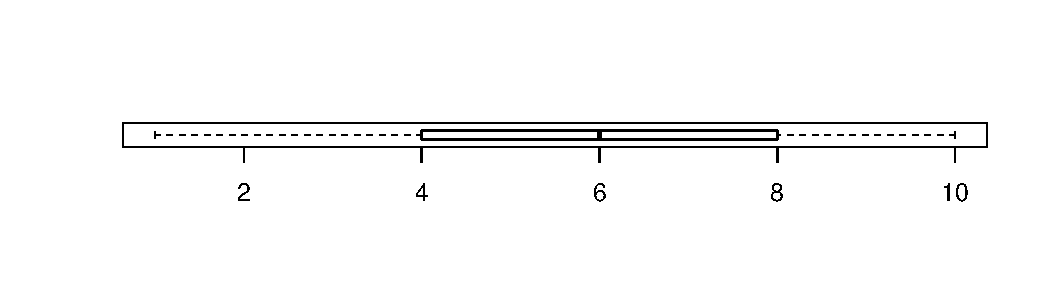
\includegraphics[width=\maxwidth]{figure/unnamed-chunk-12-1} 

\end{knitrout}


\vspace{.5cm}
(b)
Comment: Tne boxplot looks symmetric, which would be consistent with a Normal population.


(c)
Let $X_{i} \;\; i=1,\ldots,18$ be the student marks and let $\mu$ be the population mean of the marks, where $\bar{x}=5.83$ and $s=2.60$. \\

\fbox{H}
$H_0: \mu=5  \;\; vs \;\; H_1: \mu \neq 5$ \\

\fbox{A} 
Assume that $\sigma^2 = s^2 = 2.595245^2 \doteq 6.74$. \\
Note: In Tute 12 we will use the t-test instead of making this assumption. \\

 \fbox{T}
$\tau = \frac{ \bar{X} - 5}{\frac{2.595245}{\sqrt{18}}} \overset{H_0}{\sim} N(0,1) = Z$. \\
Observed value: $\tau_{0} = \frac{5.83333-5}{\frac{2.595245}{\sqrt{18}}} = 1.362307$ \\

\fbox{P} \\

Using Normal Tables: \\
$\text{P-value} = 2 P( Z > 1.36) = 2(1-P(Z < 1.36)) = 2(1-0.9131)  = 0.1738$. \\

Using R:
\begin{knitrout}
\definecolor{shadecolor}{rgb}{0.969, 0.969, 0.969}\color{fgcolor}\begin{kframe}
\begin{alltt}
\hlnum{2}\hlopt{*}\hlstd{(}\hlnum{1}\hlopt{-}\hlkwd{pnorm}\hlstd{(}\hlnum{0.3210872}\hlstd{))}
\end{alltt}
\begin{verbatim}
## [1] 0.7481443
\end{verbatim}
\end{kframe}
\end{knitrout}

\vspace{.5cm}
\fbox{C}
Since $\text{p-value} > 0.05$, we retain $H_{0}$. \\
Data is consistent with $\mu = 5$.

\vspace{1cm}
Now using $t$ test:

We have a sample with $n=50$ and $\bar{x}=1850$ and $s=110$. \\

(a)
\fbox{H}
$H_0: \mu=1800  \;\; vs \;\; H_1: \mu>1800$ \\

(b)
\fbox{A} 
We are given that the population of ropes is Normally distributed. \\

(c)
\fbox{T}
$\tau = \frac{ \bar{X} - 1800}{\frac{110}{\sqrt{50}} } \overset{H_0}{\sim}  t_{n-1} = t_{49}$. \\
Observed value: $\tau_{0} = \frac{1850-1800}{\frac{110}{\sqrt{50}} } = 3.214122 $ \\

(d)
\fbox{P} \\

Using t Tables: \\
$\text{P-value} = P( t_{49} > 3.214122 ) \approx  P( t_{50} > 3.214122 ) \; \in \; (0.001,0.0025)$. \\

\begin{knitrout}
\definecolor{shadecolor}{rgb}{0.969, 0.969, 0.969}\color{fgcolor}\begin{kframe}
\begin{alltt}
\hlstd{t}\hlkwb{=}\hlstd{(}\hlnum{1850}\hlopt{-}\hlnum{1800}\hlstd{)}\hlopt{/}\hlstd{(}\hlnum{110}\hlopt{/}\hlkwd{sqrt}\hlstd{(}\hlnum{50}\hlstd{))}
\hlnum{1}\hlopt{-}\hlkwd{pt}\hlstd{(t,}\hlnum{49}\hlstd{)}
\end{alltt}
\begin{verbatim}
## [1] 0.001158166
\end{verbatim}
\end{kframe}
\end{knitrout}

\vspace{.5cm}
(e)
\fbox{C}
Since $\text{p-value} << 0.05$, we strongly reject $H_{0}$. \\
There appears to be strong evidence that the rope strength has increased.

\end{solution}



\question 
A standard manufacturing process produces items whose lengths in mm are normally distributed with mean $\mu=10$ and standard deviation $\sigma=0.051$. A new, cheaper manufacturing process is being tested, but a manager is worried that the new process makes the items too short. A sample of 100 items produced by the new process has average length $\bar{x}=9.9921$. Assume the variability in lengths of the new process is the same as the old.  Perform a statistical test to address the manager's concerns. 


\begin{solution}
Let $X_{i} \;\; i=1,\ldots,18$ be the item lengths and let $\mu$ be the population mean of the lengths and $\sigma=0.051$. The sample of $n=100$ gives $\bar{x}=9.9921$.\\

\fbox{H}
$H_0: \mu=10  \;\; vs \;\; H_1: \mu < 10$ \\

\fbox{A} 
We assume that $\sigma = 0.051$ (as `variability of lengths of the new process is the same as the old').  \\

 \fbox{T}
$\tau = \frac{ \bar{X} - 10}{\frac{0.051}{\sqrt{100}}} \overset{H_0}{\sim} N(0,1) = Z$. \\
Observed value: $\tau_{0} = \frac{9.9921-10}{\frac{0.051}{\sqrt{100}}} = \frac{9.9921-10}{0.0051}=  -1.54902$ \\

\fbox{P} \\

Using Normal Tables: \\
$\text{P-value} = P( Z < -1.55) = 1-P(Z < 1.55) = 1-0.9394  = 0.0606$. \\

\begin{knitrout}
\definecolor{shadecolor}{rgb}{0.969, 0.969, 0.969}\color{fgcolor}\begin{kframe}
\begin{alltt}
\hlkwd{pnorm}\hlstd{(}\hlopt{-}\hlnum{1.55}\hlstd{)}
\end{alltt}
\begin{verbatim}
## [1] 0.06057076
\end{verbatim}
\end{kframe}
\end{knitrout}

\vspace{.5cm}
\fbox{C}
Since $\text{p-value} > 0.05$ (just), we retain $H_{0}$. \\
There is not enough evidence to suggest that the manager's claim is founded. However, there is a slight indication that further research might be worthwhile.
\end{solution}



\question 

A random sample of size 64 from a $N(\mu,16)$ population
yields a sample mean of 19.1. Test $H_0\colon\mu=20$ against
$H_1\colon\mu<20$. Write all your steps.


\begin{solution}
Let $X_{i} \;\; i=1,\ldots,64$ be the sample and let $\mu$ be the population mean with $\sigma^2=16$. The sample of $n=64$ gives $\bar{x}=19.1$.\\

\fbox{H}
$H_0: \mu=20  \;\; vs \;\; H_1: \mu < 20$ \\

\fbox{A} 
We are given $\sigma = 4$. \\

 \fbox{T}
$\tau = \frac{ \bar{X} - 20}{\frac{4}{\sqrt{64}}} = \frac{ \bar{X} - 20}{0.5} \overset{H_0}{\sim} N(0,1) = Z$. \\
Observed value: $\tau_{0} = \frac{19.1-20}{0.5} = -1.8$ \\

\fbox{P} \\

Using Normal Tables: \\
$\text{P-value} = P( Z < -1.8) = 1-P(Z < 1.8) = 1-0.9641  = 0.0359$. \\

\begin{knitrout}
\definecolor{shadecolor}{rgb}{0.969, 0.969, 0.969}\color{fgcolor}\begin{kframe}
\begin{alltt}
\hlkwd{pnorm}\hlstd{(}\hlopt{-}\hlnum{1.8}\hlstd{)}
\end{alltt}
\begin{verbatim}
## [1] 0.03593032
\end{verbatim}
\end{kframe}
\end{knitrout}

\vspace{.5cm}
\fbox{C}
Since $\text{p-value} < 0.05$, we reject $H_{0}$ in favour of $H_{1}$. \\
\end{solution}





\question 

A sample of size 22, from a normal population with known
variance of 2.25,  yields a total of 250.  Find an estimate of
 the population mean $\mu$.
Test the hypothesis that the
population mean $\mu$ is 10 against the alternative that the mean
is greater than 10. Write all your steps.

\begin{solution}
Let $X_{i} \;\; i=1,\ldots,22$ be the sample and let $\mu$ be the population mean with $\sigma^2=2.25$. The sample of $n=22$ gives $\sum_{i=1}^{22} x_{i}=250$.\\

\fbox{H}
$H_0: \mu=10  \;\; vs \;\; H_1: \mu > 10$ \\

\fbox{A} 
We are given $\sigma^2 = 2.25$. \\

 \fbox{T}
$\tau = \frac{ \bar{X} - 10}{\frac{\sqrt{2.25}}{\sqrt{22}}} \overset{H_0}{\sim} N(0,1) = Z$. \\
Observed value: $\tau_{0} = \frac{\frac{250}{22}-10}{\frac{\sqrt{2.25}}{\sqrt{22}}} = 4.26$ \\

\fbox{P} \\

Using Normal Tables: \\
$\text{P-value} = P( Z >4.26) = 1-P(Z < 4.26) \approx  1-0.9986  = 0.0014$. \\

\begin{knitrout}
\definecolor{shadecolor}{rgb}{0.969, 0.969, 0.969}\color{fgcolor}\begin{kframe}
\begin{alltt}
\hlnum{1}\hlopt{-}\hlkwd{pnorm}\hlstd{(}\hlnum{3.5}\hlstd{)}
\end{alltt}
\begin{verbatim}
## [1] 0.0002326291
\end{verbatim}
\end{kframe}
\end{knitrout}

\vspace{.5cm}
\fbox{C}
Since $\text{p-value} << 0.05$, we reject $H_{0}$ in favour of $H_{1}$. \\
\end{solution}





\question 

Suppose that $X_1,X_2,...,X_{49}$ are a $N(\mu,10^2)$ random sample, for some unknown $\mu$. Test the hypothesis $H_0 : \mu = 50$ against the alternative $H_1 : \mu < 50$ based on an observed value  $ \bar{x} = 48.8$, being sure to give a sensible interpretation of your p-value. Write down all your steps.


\begin{solution}
Let $X_{i} \;\; i=1,\ldots,49$ be the sample and let $\mu$ be the population mean with $\sigma^2=10^2$. The sample of $n=49$ gives $\bar{x} = 48.8$.\\

\fbox{H}
$H_0: \mu=50  \;\; vs \;\; H_1: \mu < 50$ \\

\fbox{A} 
We are given $\sigma^2 = 10^2$. \\

 \fbox{T}
$\tau = \frac{ \bar{X} - 50}{\frac{10}{7}} \overset{H_0}{\sim} N(0,1) = Z$. \\
Observed value: $\tau_{0} = \frac{48.8-50}{10/7} = -0.84$ \\

\fbox{P} \\

Using Normal Tables: \\
$\text{P-value} = P( Z < -0.84) = 1-P(Z < 0.84) = 1-0.7995  = 0.2005$. \\

\begin{knitrout}
\definecolor{shadecolor}{rgb}{0.969, 0.969, 0.969}\color{fgcolor}\begin{kframe}
\begin{alltt}
\hlkwd{pnorm}\hlstd{(}\hlopt{-}\hlnum{0.84}\hlstd{)}
\end{alltt}
\begin{verbatim}
## [1] 0.2004542
\end{verbatim}
\end{kframe}
\end{knitrout}

\vspace{.5cm}
\fbox{C}
Since $\text{p-value} > 0.05$, we retain $H_{0}$. \\

\end{solution}



\question

In accordance with the standards established for a reading comprehension test, year 8 students should average a score of 84.3 on a standard test with a standard deviation of 8.6. If 36 randomly selected eighth graders (from a school district in a low socio-economic area) averaged only 80.8, is there strong evidence that the average in that area is below standard, if it is assumed that the standard deviation for this area is 8.6, in accordance with the standard for eighth graders?


\begin{solution}
Let $X_{i} \;\; i=1,\ldots,36$ be the sample and let $\mu$ be the population mean with $\sigma^2=8.6^2$. The sample of $n=49$ gives $\bar{x} = 80.8$.\\

\fbox{H}
$H_0: \mu=84.3  \;\; vs \;\; H_1: \mu < 84.3$ \\

\fbox{A} 
We are given $\sigma = 8.6$. \\

 \fbox{T}
$\tau = \frac{ \bar{X} - 84.3}{\frac{8.6}{6}} \overset{H_0}{\sim} N(0,1) = Z$. \\
Observed value: $\tau_{0} = \frac{80.8-84.3}{8.6/6} = -2.44186$ \\

\fbox{P} \\

Using Normal Tables: \\
$\text{P-value} = P( Z < -2.44) = 1-P(Z < 2.44) = 1-0.9927  = 0.0073$. \\

\begin{knitrout}
\definecolor{shadecolor}{rgb}{0.969, 0.969, 0.969}\color{fgcolor}\begin{kframe}
\begin{alltt}
\hlkwd{pnorm}\hlstd{(}\hlopt{-}\hlnum{2.44}\hlstd{)}
\end{alltt}
\begin{verbatim}
## [1] 0.007343631
\end{verbatim}
\end{kframe}
\end{knitrout}

\vspace{.5cm}
\fbox{C}
Since $\text{p-value} << 0.05$, we reject $H_{0}$ in favour of $H_{1}$. \\
It seems that reading in the low socio-economic area is below average.
\end{solution}


\question 

\begin{parts}
\part Find $P(t_{5} \geq 3.365)$.

\part Find $P(t_{4} \leq 0.741)$.

\part Find $P(t_{7} \geq 1)$.

\part Find $a$, if $P(t_{10} \geq a) = 0.005$.

\part Find $b$, if $P(t_{10} \geq b) = 0.9$.

\end{parts}


\begin{solution}
Note: For all these questions, draw a sketch of the relevant t distribution. This is particularly important for (e), so that you get the right sign. \\


(a) 
$P(t_{5} \geq 3.365) = 0.01$ (from t table). \\

\begin{knitrout}
\definecolor{shadecolor}{rgb}{0.969, 0.969, 0.969}\color{fgcolor}\begin{kframe}
\begin{alltt}
\hlnum{1}\hlopt{-}\hlkwd{pt}\hlstd{(}\hlnum{3.365}\hlstd{,}\hlnum{5}\hlstd{)}
\end{alltt}
\begin{verbatim}
## [1] 0.009999236
\end{verbatim}
\end{kframe}
\end{knitrout}

\vspace{.5cm}
(b)
$P(t_{4} \leq 0.741) = 0.75$.  \\
Note that the t table is upper tail, so we calculate 1-0.25. \\

\begin{knitrout}
\definecolor{shadecolor}{rgb}{0.969, 0.969, 0.969}\color{fgcolor}\begin{kframe}
\begin{alltt}
\hlkwd{pt}\hlstd{(}\hlnum{0.741}\hlstd{,}\hlnum{4}\hlstd{)}
\end{alltt}
\begin{verbatim}
## [1] 0.7500824
\end{verbatim}
\end{kframe}
\end{knitrout}

\vspace{.5cm}
(c)
$P(t_{7} \geq 1) \in (0.1,0.25)$. \\
Note that 1 is between 0.711 and 1.415, hence from the table, we can only say that the probability is in the interval $(0.1,0.25)$.
Using R, we can get the exact value. \\

\begin{knitrout}
\definecolor{shadecolor}{rgb}{0.969, 0.969, 0.969}\color{fgcolor}\begin{kframe}
\begin{alltt}
\hlnum{1}\hlopt{-}\hlkwd{pt}\hlstd{(}\hlnum{1}\hlstd{,}\hlnum{7}\hlstd{)}
\end{alltt}
\begin{verbatim}
## [1] 0.1753083
\end{verbatim}
\end{kframe}
\end{knitrout}


\vspace{.5cm}
(d)
From the t table, we can see that $P(t_{10} \geq 3.169) = 0.005$, hence $b=3.169$. \\

\begin{knitrout}
\definecolor{shadecolor}{rgb}{0.969, 0.969, 0.969}\color{fgcolor}\begin{kframe}
\begin{alltt}
\hlkwd{qt}\hlstd{(}\hlnum{.995}\hlstd{,}\hlnum{10}\hlstd{)}
\end{alltt}
\begin{verbatim}
## [1] 3.169273
\end{verbatim}
\end{kframe}
\end{knitrout}


\vspace{.5cm}
(e) Find $b$, if $P(t_{10} \geq b) = 0.9$.

From the t table, we can see that $P(t_{10} \geq 1.372) = 0.1$. \\
Hence by symmetry,  $P(t_{10} \leq -1.372) = 0.1$. \\
Hence by symmetry,  $P(t_{10} \geq -1.372) = 0.9$. \\
So $b=-1.372$. \\

\begin{knitrout}
\definecolor{shadecolor}{rgb}{0.969, 0.969, 0.969}\color{fgcolor}\begin{kframe}
\begin{alltt}
\hlkwd{qt}\hlstd{(}\hlnum{0.1}\hlstd{,}\hlnum{10}\hlstd{)}
\end{alltt}
\begin{verbatim}
## [1] -1.372184
\end{verbatim}
\end{kframe}
\end{knitrout}

\end{solution}

\question 

A new measuring technique is being considered to replace the standard technique. When 10 samples are measured by both techniques, the measurements are: \\
\begin{center}
\begin{tabular}{|l|cccccccccc|}\hline
 Sample &1&2&3&4&5&6&7&8&9&10\\ \hline
New Technique     &2.5 &2.2 &2.6 &2.6 &1.9 &3.3 &3.3 &2.8 &3.0 &2.9\\
Standard Technique &2.1 &2.4 &2.1 &1.9 &2.0 &2.8 &2.7 &2.8 &2.8 &3.0\\ \hline
Difference & & & & & & & & & & \\ \hline
\end{tabular}
 \end{center}

\begin{parts}
\part Show that the mean and the standard deviation of the differences (New -Standard) are 0.25 and 0.331. Assuming that the differences are normally distributed, test the hypothesis that the techniques give the same results.

\part Produce a boxplot of the differences. Comment.

\part  (Revision of Week 9)
Test the hypothesis that there is no long-run systematic difference between the two techniques %give the same results 
using a sign test.

\end{parts}


\begin{solution}
(a)

\begin{tabular}{|l|cccccccccc|}\hline
 Sample &1&2&3&4&5&6&7&8&9&10\\ \hline
New Technique     &2.5 &2.2 &2.6 &2.6 &1.9 &3.3 &3.3 &2.8 &3.0 &2.9\\
Standard Technique &2.1 &2.4 &2.1 &1.9 &2.0 &2.8 &2.7 &2.8 &2.8 &3.0\\ \hline
Difference & 0.4 & -0.2 & 0.5 & 0.7 & -0.1 & 0.5 & 0.6 & 0 & 0.2 & -0.1 \\ \hline
\end{tabular}

\vspace{.5cm}
\begin{verbatim}
> a=c(2.5,2.2,2.6,2.6,1.9,3.3,3.3,2.8,3.0,2.9)
> a
 [1] 2.5 2.2 2.6 2.6 1.9 3.3 3.3 2.8 3.0 2.9
> b=c(2.1,2.4,2.1,1.9,2.0,2.8,2.7,2.8,2.8,3.0)
> diff=a-b
> diff
 [1]  0.4 -0.2  0.5  0.7 -0.1  0.5  0.6  0.0  0.2 -0.1
[1] 0.25
> sd(diff)
[1] 0.3308239
\end{verbatim}

\vspace{.5cm}
\fbox{H}
$H_0: \mu_{d}=0  \;\; vs \;\; H_1: \mu_{d} \neq 0$ \\

\fbox{A} 
We assume that the population is Normally distributed. \\

\fbox{T}
$\tau = \frac{ \bar{X} - 0 }{ \frac{0.3308239}{\sqrt{10}}   }   \overset{H_0}{\sim}  t_{n-1} = t_{9}$. \\
Observed value: $\tau_{0} = \frac{0.25-0}{\frac{0.3308239}{\sqrt{10}} }  \doteq  2.39 $ \\

\fbox{P} \\

Using t Tables: \\
$\text{P-value} = 2 P( t_{9} >  2.39 ) \; \in \; (0.02,0.05)$. \\

\vspace{.5cm}
\fbox{C}
Since $\text{p-value} < 0.05$, we would reject $H_{0}$ at $\alpha = 0.05$. \\
The new technique does seem to be significantly different from the standard technique. \\

(b)
Comment: Boxplot is fairly symmetric, so Normality assumption for t Test seems appropriate. 


(c)
\fbox{Preparation} \\
The signs of differences are: 
$\{ + - + + - + +  \; 0 +  -\}$. \\

$X = \text{Number of $+$ signs} \sim Bin(9, p)$, where $\rho = P(\text{preference for New Technique})$. \\
Note: 1 reading was discarded, so we have $n= 9$ and $x=6$. \\

\fbox{H} 
$H_0: \rho=0.5  \;\; vs \;\; H_1: \rho \neq 0.5$ \\

\fbox{A} We assume the results were sampled independently with same $\rho$. \\

\fbox{T} 
$X \overset{H_0}{\sim} Bin(9,0.5)$.\\
Observed value: $x=6$. \\

\fbox{P}
$\text{P-value} = 2 P(X \geq 6) = 2(1- P(X \leq 5) 
= 2(1- 0.7461) =  0.5078$. \\

\fbox{C} As $\text{p-value} >> 0.05$, the evidence is consistent with $H_{0}$. \\
Hence, there is not evidence of difference in techniques. \\

Note: Here we get a different conclusion from the t Test. The reason is that the Sign Test only uses the signs (not magnitudes) of differences. We can see that the positive differences are much bigger than the negative ones, and this is lost in the Sign test. Hence, it would better to use the t Test.
\end{solution}



\end{questions}
\end{tutorial}
\end{document}
